%% Computational Linguistics -- Short Paper submission.
%%
%% Build:  latexmk -pdf cl-short-paper.tex   (from paper/)
%% Figures: reports/figures/cl/  Tables: reports/tables/cl/   Bibliography: bibs/cl-short-paper.bib
%% Both are regenerated from tracked artefacts by scripts/cl_paper/.

\documentclass[final]{clv2025}

\jvol{vv}
\jnum{nn}
\jyear{2026}
% There is no need for the authors to change the above.

\dochead{Short Paper}

\pageonefooter{Action editor: \{action editor name\}. Submission received: DD Month YYYY; revised version received: DD Month YYYY; accepted for publication: DD Month YYYY.}

\usepackage{amsmath}
\usepackage{booktabs}
\usepackage{graphicx}

\graphicspath{{../reports/figures/cl/}}

\runningtitle{Measurement Invariance in Lexical Semantic Change}
\runningauthor{L\"utkemeier}

\begin{document}

\title{Is Lexical Semantic Change Measurement-Invariant?\\ Lexicon, Encoder, and Discourse Composition\\ in a Web-Scale Study of ADHD and Autism}

\author{Jakob L\"utkemeier}

\affilblock{
    \affil{Trinity College Dublin, School of Social Sciences and Philosophy\\\quad \email{jakob.luetkemeier@gmail.com}}
}

% The class writes the page-one footer through \@footnotetext, which reads \@thefnmark.
% That macro is only defined as a side effect of \thanks, so a paper with no \thanks --
% such as this single-author one -- would otherwise fail at \maketitle.
\makeatletter
\providecommand{\@thefnmark}{}

% \appendixsection uses \section*, which never runs \refstepcounter, so a \label placed
% after it would capture whatever counter was stepped last and print an arabic numeral
% instead of the appendix letter. \applabel binds the label to \Alph{section} explicitly.
\newcommand{\applabel}[1]{%
  \protected@edef\@currentlabel{\Alph{section}}%
  \label{#1}%
}

% \appendixsection resets the table and figure counters per appendix, so hyperref's
% anchor names collide across appendices unless the section letter is folded into the
% hypertext counters as well as the printed ones. Setting them at each \appendixsection
% (rather than at \begin{document}) keeps them from being overwritten by hyperref's own
% begin-document hook.
\let\cl@appendixsection\appendixsection
\renewcommand{\appendixsection}[1]{%
  \cl@appendixsection{#1}%
  \renewcommand{\theHtable}{\Alph{section}.\arabic{table}}%
  \renewcommand{\theHfigure}{\Alph{section}.\arabic{figure}}%
}
\makeatother

\maketitle

\begin{abstract}
Diachronic measures of lexical semantic change are increasingly used to license claims
about cultural change, but those claims inherit whatever the instrument does. We ask
whether two such threats---dependence on the resources chosen to operationalise a
dimension, and confounding with change in discourse composition---are large enough to
alter published conclusions. Building a 13-year corpus of general web discourse from
Common Crawl and stratifying 96{,}864 target mentions by discourse frame with an
LLM-in-the-loop classifier, we estimate annual sentiment, intensity, and breadth
trajectories for two diagnostic concepts, ADHD and autism, against three
negative-emotion comparators, and then re-estimate every trajectory under the alternative
lexicon and encoder that the same framework originally specified. Fifteen of twenty-seven
series change their descriptive conclusion, and the failures are dimension-specific:
sentiment is close to invariant while intensity and breadth are not. Crossing the two
lexicons shows why---they agree about valence and disagree about arousal on the same
tokens---and a perturbation probe shows the two encoders differ by an order of magnitude in
how much non-target material moves them. Substantively, neither predicted form of concept
creep is supported, and a shift-share decomposition shows the null is conservative: the
corpus composition was drifting in the direction that manufactures apparent creep. We argue
that multi-resource comparison and composition stratification belong in the primary
analysis of semantic change, not in a robustness appendix.
\end{abstract}

\keywords{lexical semantic change; diachronic NLP; measurement validity; discourse
composition; contextual embeddings; Common Crawl; corpus construction; LLM-assisted
annotation; concept creep}

\section{Introduction}

Computational studies of lexical semantic change (LSC) are increasingly asked to do
cultural work. Having established that meaning change can be detected at scale
\citep{hamilton-etal-2016-diachronic,schlechtweg-etal-2020-semeval}, the field is now
routinely used to argue that a society's concepts of harm, illness, or identity have
shifted \citep{vylomovaSemanticChangesHarmrelated2021,baesSemanticShiftsMental2023}. That
is a considerable inferential burden for a measurement to carry, and it makes the
properties of the measurement itself a first-order question. A trend estimated from
lexicon-weighted collocates or embedding dispersion is only evidence about a concept if it
is stable under choices that were never meant to be substantive.

Two such threats are well known individually and rarely tested together. The first is
\emph{operationalisation dependence}. LSC estimates have repeatedly proved sensitive to
things that ought not to matter: the random seed and corpus slice used to fit embeddings
\citep{antoniak-mimno-2018-evaluating}, the frequency and polysemy profile of the target
against a proper control \citep{dubossarsky-etal-2017-outta}, and even orthographic
preprocessing before a contextual encoder \citep{laicher-etal-2021-explaining}. The second
is \emph{discourse-composition confounding}. A word's measured context can change because
its meaning changed, or because the population of texts that use it changed. Working on
newspaper text, \citet{pislRevisitingSemanticSeverity2025} showed that an apparent
semantic-intensity trend for \emph{depression} became non-significant once the balance of
clinical and non-clinical contexts was controlled.

We test both in a single design, on a case that carries a strong standing directional
prediction. Concept creep theory holds that harm-related concepts broaden to admit
qualitatively new instances (horizontal creep) and loosen to admit milder ones (vertical
creep) \citep{haslamConceptCreepPsychologys2016,haslamHarmInflationMaking2020}, and a
series of studies reports exactly that for mental-health vocabulary
\citep{vylomovaSemanticChangesHarmrelated2021,baesSemanticInflationTrauma2023,baesSemanticShiftsMental2023}.
ADHD and autism are useful test cases: they are unambiguously diagnostic concepts, so the
polysemy that complicates \emph{depression} or \emph{anxiety} does not arise
\citep{xiaoHaveConceptsAnxiety2023}, and they sit at the centre of contemporary argument
about whether the popularisation of clinical language erodes its meaning
\citep{isern-masUnmaskingTherapyspeak2025,spencerIsntEveryoneLittle2021}. If a
directional prediction of this strength cannot be evaluated invariantly, weaker ones
cannot either.

The paper makes five contributions.

\begin{enumerate}
\item A reusable pipeline for constructing diachronic corpora of general web discourse
from Common Crawl, using a WET-first scan with WARC-validated extraction, applied here to
13 annual snapshots from 2014 to 2026 (Section~\ref{sec:corpus}).

\item A frame-aware design that separates discourse composition from meaning before trends
are estimated, with frame labels produced by an LLM annotator under critical review and
human adjudication (LLM--human $\kappa$ between .87 and .95) and audited for temporal
stability (Section~\ref{sec:design}).

\item Evidence that the intensity and breadth dimensions of a published LSC framework are
not measurement-invariant, while its sentiment dimension largely is: substituting the
framework's own original lexicon and encoder changes the descriptive conclusion for 15 of 27
series, concentrated in two of the three dimensions. This holds for the comparator terms as
well as the targets, so it is not an artefact of the case (Section~\ref{sec:sensitivity}).

\item An account of \emph{why} each substitution matters: crossing the two lexicons
attributes their disagreement to ratings rather than coverage, and a perturbation probe
shows the two encoders differ by an order of magnitude in how much non-target material
moves their representations (Section~\ref{sec:mechanism}).

\item A bounded null result for concept creep in two institutionally codified diagnostic
concepts, with the smallest detectable linear changes stated explicitly
(Sections~\ref{sec:vertical}--\ref{sec:horizontal}).

\end{enumerate}

Code, configuration, and the derived annual estimates behind every figure and table are
available at \url{https://github.com/jako6f/msc-nlp-therapy-speak}.

\section{Background}

\subsection{Measuring Lexical Semantic Change}

Computational LSC detection has moved through three broad representations
\citep[for surveys see][]{tahmasebiSurveyComputationalApproaches2019,tangStateoftheartSemanticChange2018,kutuzovDiachronicWordEmbeddings2018,peritiMontanelliLSCSurvey2024,saSurveyCharacterizingSemantic2026}.
Type-level embeddings assign one vector per word per period and compare them across
aligned spaces \citep{hamilton-etal-2016-diachronic,mikolovDistributed2013}. Contextual
embeddings assign a vector per usage, so change can be characterised as a shift in the
distribution of usages rather than in a single point
\citep{giulianelli-etal-2020-analysing}. Target-aware word-in-context models go further
and encode the target occurrence specifically, which is what the word-in-context task
requires \citep{pilehvar-camacho-collados-2019-wic}; XL-LEXEME is trained for exactly this
and is the current default for LSC detection \citep{cassottiXLLEXEMEWiCPretrained2023}.

Alongside this progress runs a persistent methodological worry. Embedding-derived
similarity is unstable across corpus samples and initialisations
\citep{antoniak-mimno-2018-evaluating}; apparent ``laws'' of semantic change partly reflect
frequency and polysemy artefacts that only proper controls reveal
\citep{dubossarsky-etal-2017-outta}; results differ across corpora and time spans for the
same targets \citep{schlechtweg-etal-2019-wind}; and even preprocessing decisions upstream
of a contextual encoder move measured change substantially
\citep{laicher-etal-2021-explaining}.

These results share a structure worth making explicit, because it shapes what we test
here. Each identifies a degree of freedom that the analyst does not experience as a
substantive choice---a seed, a sampling window, a normalisation step---and shows that it
moves the estimate. But each also concerns the \emph{detection} stage: whether a word
changed, and by how much. The frameworks now being used to make cultural arguments add a
second stage on top of detection, in which change is decomposed into interpretable
dimensions and each dimension is estimated from a designated resource---an affect lexicon,
an encoder. That second stage introduces degrees of freedom of its own, and they have not
been probed in the same way. Two questions follow, and we take both. Does substituting a
resource that the framework's own authors treat as interchangeable reverse a substantive
finding? And if so, can the mechanism be identified well enough that a practitioner using a
single resource could detect their own exposure to it?

\subsection{Characterising Change: The SIBling Framework}

Most LSC work asks \textit{whether} a word changed. \citet{baesMultidimensionalFrameworkEvaluating2024}
ask \textit{how}, proposing the SIBling framework---Sentiment, Intensity, Breadth---to characterise
change along interpretable dimensions rather than as one aggregate distance. Sentiment and
intensity are estimated as the mean valence and arousal of affect-rated collocates in a
local window; breadth is the mean pairwise distance among contextual embeddings of the
target's usages. The three dimensions map onto the LSC vocabulary of amelioration and
pejoration, of strengthening and weakening, and of narrowing and broadening
\citep{campbellHistoricalLinguisticsIntroduction2013}, and the framework is explicitly
offered to social scientists as a way to make cultural inferences from lexical evidence.

The authors describe their operationalisations as first implementations that have not been
externally validated and remain open to refinement. This paper takes that caveat as a
research question. Two substitutions are natural. For affect, the Warriner norms
\citep{warrinerNorms2013} used in the original can be replaced by NRC--VAD v2.1
\citep{mohammadNRCVADLexicon2025}, which offers roughly threefold lexical coverage,
multi-word entries, and higher reported reliability. For breadth, the generic sentence
encoder \citep{songMPNet2020,reimers-gurevych-2019-sentence} can be replaced by a
target-aware model \citep{cassottiXLLEXEMEWiCPretrained2023}, on the argument that the
analytic object is a term's usage rather than a document's topic. Both substitutions are
defensible \emph{a priori}. The empirical question is whether choosing between them
changes what one concludes.

\subsection{The Hypothesis Under Test}

Concept creep theory predicts that harm-related concepts loosen vertically and broaden
horizontally over time \citep{haslamConceptCreepPsychologys2016,haslamConceptCreepMental2026}.
Concepts of mental illness qualify as harm-related because distress and dysfunction are
central to their definition \citep{wakefieldConceptMentalDisorder1992}. The evidence base is
substantial but mixed. Creep has been reported for \emph{trauma}, \emph{addiction},
\emph{bullying}, \emph{prejudice}, and \emph{harassment} in psychology abstracts and in
curated general-language corpora
\citep{vylomovaSemanticChangesHarmrelated2021,baesSemanticShiftsMental2023}. Against this,
\citet{xiaoHaveConceptsAnxiety2023} found the semantic intensity of \emph{anxiety} and
\emph{depression} \emph{increasing}, and \citet{iacobComputationalAnalysisEmergence2026}
found most therapy-speak terms broadening in psychology abstracts but narrowing on Reddit,
with long-established clinical terms barely moving at all.

Two features of this record motivate our design. First, it rests almost entirely on
curated corpora, whose composition reflects editorial and disciplinary conventions as much
as public usage; general web discourse has not been examined systematically, despite being
the substrate from which large-scale corpora are now routinely built
\citep{wenzekCCNetExtractingHigh2019,penedoFineWeb2024}. Second, the divergent findings are consistent with
both threats we test: they could reflect real differences between concepts, or shifting
composition, or instrumentation. The compositional threat has a specific and directional
form here. Clinical contexts are affectively more intense than lived-experience ones, so a
corpus whose mixture drifts toward clinical language will show rising measured intensity and
one drifting away from it will show falling intensity, whichever way the meaning of the term
is moving. A drift of the first kind is what this literature calls \emph{pathologisation},
and measures of it have been built directly into the collocate-based tradition
\citep{baesSemanticShiftsMental2023,baesMultidimensionalFrameworkEvaluating2024}. An
aggregate estimate conflates pathologisation with semantic change unless the mixture is
modelled, which is precisely the confound \citet{pislRevisitingSemanticSeverity2025}
identify for \emph{depression} in newspaper text.

We therefore evaluate the two directional creep hypotheses---declining intensity and
increasing breadth for ADHD and autism---as the substantive test, and treat sentiment and
frame composition as exploratory.

\section{Corpus Construction}
\label{sec:corpus}

\subsection{Common Crawl as an Evidentiary Base}

Common Crawl is the largest openly available web archive, published roughly monthly with
more than two billion pages per crawl \citep{CommonCrawlGet}. Its value here is breadth: it
provides repeated cross-sections of general web discourse rather than one platform or
newspaper archive.

Its limits should be stated before its results, not after. Common Crawl is neither a
complete copy of the web nor a representative sample of it \citep{baackCriticalAnalysisLargest2024}.
Since 2017 domain selection has followed harmonic centrality, so well-linked domains are
both likelier to be crawled and more deeply crawled; large social platforms are absent;
and rights-holder blocking via \texttt{robots.txt} has grown over precisely the years we
study. Temporal comparability is therefore imperfect by construction. Following the spirit
of data statements \citep{bender-friedman-2018-data,elazarWIMBD2024}, we take the corpus to
license claims about quality-filtered, English-language open-web discourse as archived by
Common Crawl, and about nothing wider.

\begin{figure}[t!]
\begin{center}
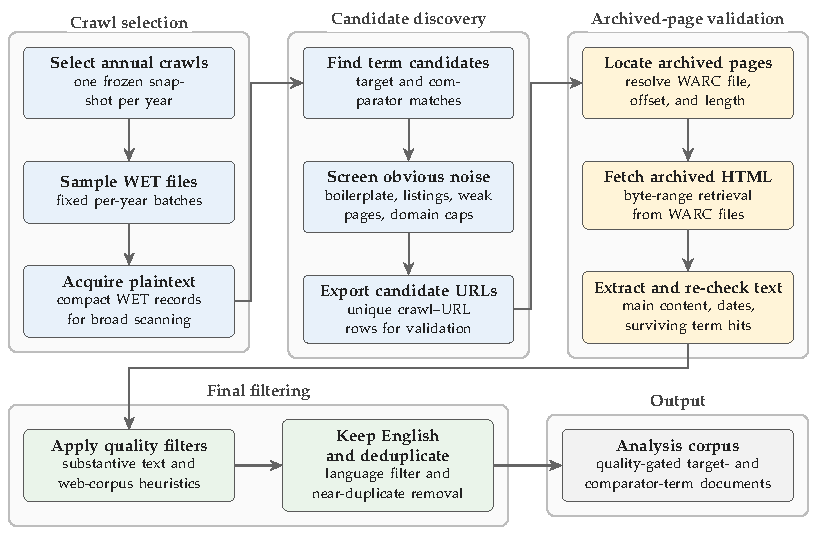
\includegraphics[width=\textwidth]{fig1_pipeline.pdf}
\end{center}
\caption{The collection pipeline. \emph{Crawl selection} freezes one snapshot per year and
acquires its compact WET plaintext. \emph{Candidate discovery} scans that plaintext for
target and comparator matches, screens obvious noise, and exports candidate URLs.
\emph{Archived-page validation} resolves each candidate to its WARC record, fetches the
original HTML by byte range, and re-extracts main text, dates, and surviving term hits.
\emph{Final filtering} applies document-quality gates, an English filter, and near-duplicate
removal, yielding the quality-gated analysis corpus. Reserving the expensive WARC stage for
candidates only is what makes web-scale diachronic collection affordable.}
\label{fig:pipeline}
\end{figure}

\subsection{Pipeline}

Figure~\ref{fig:pipeline} shows the collection design. It exploits the two Common Crawl
formats sequentially. WET files hold compact extracted plaintext and are cheap to scan, so
they carry large-scale term matching; but they lack the HTML structure needed for
boilerplate removal and metadata recovery. Candidate documents
are therefore resolved to their WARC records, where the original HTML is fetched by byte
range and main text re-extracted. Reserving WARC processing for candidates only is what
makes web-scale diachronic collection affordable: the full run scanned 220 million pages on
a single two-vCPU cloud instance at roughly one hour per million WET records.

Software choices affect corpus membership and are therefore reported. WET and WARC records
are parsed with \texttt{warcio}; WARC pointers resolve through a local \texttt{pywb} index
server; archived HTML is converted to main text with Trafilatura and Resiliparse
\citep{barbaresiTrafilaturaWebScraping2021,bevendorffElasticChatNoirSearch2018};
publication dates are recovered with \texttt{htmldate}
\citep{barbaresiHtmldatePythonPackage2020}; and post-extraction filtering applies DataTrove
quality filters \citep{penedoDataTroveLargeScale2026} followed by language identification
with \texttt{py3langid} \citep{luiLangidpyOfftheshelfLanguage2012}. One crawl is selected
per year near a fixed anchor date and frozen in a crawl map, so the sampling frame is
deterministic and re-runnable. To limit domination by large sites beyond Common Crawl's own
sampling, we cap retained hits at 50 rows per registered domain per crawl.

Across 2014--2026 the collection scanned 220 million pages and retained 336{,}178
analysis-ready documents, of which 87{,}173 contain an ADHD or autism term.

\subsection{Targets, Comparators, and Contexts}

% Long verbatim tokens cannot be hyphenated and force very loose lines in a 32pc measure.
% \pat marks a break opportunity inside each expression.
\newcommand{\pat}[1]{\texttt{#1}\allowbreak}
The targets are matched with frozen expressions covering \pat{adhd} and
\pat{attention[-\textbackslash s]?}\pat{deficit} for ADHD, and \pat{autism},
\pat{autistic}, \pat{autism[-\textbackslash s]?}\pat{spectrum}, and \pat{ASD} for
autism, with \texttt{ASD} retained only when \emph{autism} occurs within $\pm200$
characters. Three negative, non-clinical emotion terms---\emph{frustration},
\emph{sadness}, \emph{loneliness}---serve as comparators. They are not matched semantic
controls in the sense of \citet{dubossarsky-etal-2017-outta}; they establish whether the
instruments detect movement at all in this corpus over this window, which is what a null
result on the targets requires.

The unit of analysis is the individual mention rather than the document. Overlapping
matches are resolved to the longest span, and same-sentence acronym--expansion pairs are
collapsed so that ``attention deficit hyperactivity disorder (ADHD)'' contributes one
context rather than two; each document may contribute at most three mentions per analysis
unit, which limits domination by repetitive documents while preserving repeated-use signal.

The attrition from documents to mentions is worth reporting, because in web corpora it is
where silent selection happens. The 336{,}178 analysis-ready documents yielded 664{,}606
raw matches; overlap resolution reduced this to 643{,}735, acronym--expansion collapse to
633{,}026, and the three-mention cap to 465{,}400 candidate contexts. The publication-year
filter then removed 161{,}122 contexts published before 2014 and 10{,}608 with no parseable
date. The large document-level attrition, from 336{,}178 to 212{,}651, therefore reflects
mostly archived pages published before the study window rather than aggressive filtering:
each yearly crawl also captures older pages. The result is 293{,}670 mention contexts from
212{,}651 documents across 135{,}771 registered domains, including 96{,}864 target contexts
(28{,}611 ADHD, 68{,}253 autism).

Each context stores a $\pm5$-token window for affective analysis and the target sentence
with adjacent context for embedding analysis. Documents may contain both
targets---11{,}795 do---and contribute separately to each, which matters for
interpretation: as the two concepts are increasingly discussed together, each becomes part
of the other's measured context \citep{kangConvergingRepresentationsAttentionDeficit2025}.

\section{Frame-Aware Design and Measures}
\label{sec:design}

\subsection{Frame Classification}
\label{sec:frames}

In web text, ADHD and autism appear as diagnoses, disorder constructs, service categories,
identities, community labels, and incidental boilerplate. Treating all mentions as one
semantic population risks reading a change in that mixture as a change in meaning. We
therefore label each target passage---the target sentence plus adjacent context---before
estimating any trend.

Labelling is hierarchical. A passage is first coded for whether it contains substantive
target discourse; passages that are thin, navigational, promotional, or otherwise
insufficient for target-specific interpretation are set aside. Substantive passages are
then coded on two non-exclusive axes: whether clinical framing is present (diagnosis,
disorder status, symptoms, impairment, treatment, services, medication, research,
epidemiology, DSM/ICD-style categories, and educational or clinical support needs) and
whether lived-experience framing is present (identity, self-understanding, family or
first-person experience, neurodivergent community, stigma, accommodation, everyday coping,
belonging, pride, and embodied or social experience).

The axes are deliberately non-exclusive, because a passage can do both---a first-person
account of receiving a diagnosis is simultaneously clinical and experiential---and forcing
a single choice would push exactly the ambiguous cases into arbitrary bins. They combine
deterministically into five derived strata: clinical but not lived (\emph{clinical-only}),
lived but not clinical (\emph{lived-only}), both (\emph{mixed}), substantive but neither
(\emph{substantive-other}), and non-substantive. The analyses report the two unambiguous
strata alongside the substantive aggregate. Mixed contexts are estimated but not plotted
separately: this smaller stratum generally tracked between the overall and clinical
trajectories and added visual overlap without changing any conclusion.

Labels were produced by an Annotation with Critical Thinking workflow
\citep{linACTHumanMultimodal2025}. A 200-passage human pilot fixed the codebook. The locked
codebook was then applied to 3{,}000 passages, stratified by year and target, by a frozen
annotator (\texttt{gpt-5.5}, accessed through the Codex CLI at high reasoning effort with
web search disabled); a second, independent model (\texttt{gemini-3-flash-preview}, accessed
through the Gemini CLI) reviewed every annotation and assigned an error-risk score; and a
human coder reviewed and corrected the 400 highest-risk cases plus a random sample of
low-risk cases. No model suggestion changed a label without human
review. This follows the emerging consensus that LLM annotation is useful but requires
validation against human judgement rather than substituting for it
\citep{gilardiChatGPT2023,pangakisValidation2023,ziems-etal-2024-large}.

The corrected labels trained a hierarchical classifier over sentence embeddings
\citep{songMPNet2020}: three balanced logistic heads, one predicting substantive discourse
over all labelled examples and two predicting the frame axes among substantive examples.
Year, URL, and domain features are excluded to avoid leakage from temporal or source
artefacts. A separate 200-passage validation set was withheld from codebook development,
LLM annotation, criticism, correction, and training.

\begin{table}[t!]
\caption{Annotation reliability and held-out classifier validation for the three
hierarchical frame decisions. LLM--human agreement compares the locked Codex annotator
against the human coder on the 200-passage pilot; classifier performance is measured on
the disjoint 200-passage validation set, which was withheld from codebook development,
LLM annotation, criticism, correction, and training.}
\label{tab:annotation}
\small
\begin{tabular}{@{}lccccccc@{}}
\toprule
& \multicolumn{3}{c}{LLM--human agreement} & \multicolumn{4}{c}{Held-out classifier} \\
\cmidrule(r){2-4}\cmidrule(l){5-8}
Decision & $n$ & Agr. & $\kappa$ & Support & P & R & F1 \\
\midrule
Substantive target discourse & 200 & .960 & .914 & 141/200 & .887 & .837 & .861 \\
Clinical framing & 122 & .943 & .867 & 105/141 & .903 & .886 & .894 \\
Lived-experience framing & 122 & .975 & .949 & 46/141 & .704 & .826 & .760 \\
\bottomrule
\end{tabular}
\par\vspace{3pt}
\parbox{\linewidth}{\footnotesize Note. The clinical and lived-experience rows are
evaluated among passages the human coder judged substantive. All human labels come from a
single coder, so no inter-annotator agreement is reportable.}
\end{table}


Table~\ref{tab:annotation} reports both halves of this instrument. The LLM annotator
agrees with the human coder closely on all three decisions: $\kappa = .914$ on whether a
passage is substantive target discourse (96.0\% raw agreement over 200 passages),
$\kappa = .867$ on clinical framing, and $\kappa = .949$ on lived-experience framing
(both over the 122 passages the coder judged substantive). Agreement on the five-way
derived stratum, which requires all three decisions to coincide, is $\kappa = .877$. These
are high enough that the LLM stage is doing recognisably the same task as the human
one, which is what licenses using it at a scale hand-coding could not reach.

The classifier trained on those labels transfers well to the held-out set. Substantive-
discourse detection reaches F1 = .861 and clinical framing F1 = .894, both close to the
agreement ceiling above. Lived-experience framing is the weakest head (F1 = .760,
precision = .704), which matters for interpretation: lived-experience strata contain
clinical admixture, so frame contrasts are attenuated and the frame-specific trends
reported below are, if anything, conservative. One caveat belongs with all of these
numbers: every human label in this study comes from a single coder, so no inter-annotator
agreement is reportable and validation is measured against an individual rather than a
consensus standard.

A post-hoc diagnostic checks the frame distinction without involving the classifier at all.
Fitting annual skip-gram models separately within each frame and extracting each target's
recurrent nearest neighbours \citep{mikolovDistributed2013,vylomovaSemanticChangesHarmrelated2021}
recovers the same division from distributional evidence alone (Appendix~\ref{app:thematic}).
For autism the two neighbour sets are almost disjoint: clinical contexts yield
\emph{developmental}, \emph{disorder}, \emph{research}, and \emph{study}, lived-experience
contexts \emph{family}, \emph{life}, \emph{people}, and \emph{support}. ADHD shows the same
contrast more weakly, with \emph{disorder}, \emph{symptom}, and \emph{condition} against
\emph{help}. The frames therefore track a real difference in how these terms are used, not
an artefact of the codebook.

\subsection{Measures}

For analysis unit $u$, publication year $Y$, and stratum $s$, \textbf{sentiment} and
\textbf{intensity} are the frequency-weighted mean valence $V(w)$ and arousal $A(w)$ of
affect-rated collocates in the $\pm5$-token windows,
\begin{equation}
\operatorname{Sentiment}_{u,Y,s} =
\frac{\sum_{w \in C_{u,Y,s}} f_{w,u,Y,s}\,V(w)}{\sum_{w \in C_{u,Y,s}} f_{w,u,Y,s}},
\quad
\operatorname{Intensity}_{u,Y,s} =
\frac{\sum_{w \in C_{u,Y,s}} f_{w,u,Y,s}\,A(w)}{\sum_{w \in C_{u,Y,s}} f_{w,u,Y,s}},
\end{equation}
where $C_{u,Y,s}$ is the set of matched collocates and $f$ their frequencies. The focal
term is removed from its own window. Windows are tokenised, tagged, and lemmatised with
spaCy \citep{honnibalSpacy2020}; punctuation, symbols, numerals, one-character lemmas, and
stopwords are excluded; lexicon entries are normalised identically, and multi-word entries
matched greedily before unigrams.

\textbf{Breadth} operationalises horizontal creep as contextual dispersion. Each context is
marked with explicit target delimiters and encoded by XL-LEXEME, and breadth is the mean
pairwise cosine distance among the $N_{u,Y,s}$ resulting L2-normalised target-use
embeddings,
\begin{equation}
\operatorname{Breadth}_{u,Y,s} =
\frac{2}{N_{u,Y,s}(N_{u,Y,s}-1)}
\sum_{i<j}\left(1 - \mathbf{v}_i \cdot \mathbf{v}_j\right).
\end{equation}
Higher values mean more heterogeneous usage. The implementation evaluates this in closed
form over the normalised vectors rather than materialising the pairwise matrix.


\subsection{Alternative Operationalisations}
\label{sec:alternatives}

Every affective and breadth trajectory is estimated twice. The primary estimates use
NRC--VAD and XL-LEXEME; the alternative estimates use the resources SIBling originally
specified, the Warriner norms and MPNet sentence embeddings, with the annual strata,
sampling, and trend-model conventions held constant.

One constraint governs how the two can be compared. The lexicons live on different native
scales---NRC--VAD spans $-1$ to $1$, the Warriner norms are a 1--9 scale rescaled to
$0$--$1$---so raw slope magnitudes are not commensurable. We therefore compare only the
\emph{sign}, the \emph{significance verdict}, and the \emph{standardised} year
coefficient, never the unstandardised slope. The MPNet breadth track is extended to the comparator
terms here, so every dimension is compared over the same set of series.

\subsection{Statistical Analysis}
\label{sec:stats}

Annual estimates are the objects of interpretation. Uncertainty intervals come from
document-level bootstrap resampling within each unit--year--stratum cell (500 repetitions,
2.5th and 97.5th percentiles); the document is the resampling unit because mentions and
collocates from one document are not independent. Ordinary least squares over the 13 annual
points summarises net linear movement. Residual autocorrelation is assessed with a
Durbin--Watson statistic and flagged outside $[1.25, 2.75]$; flagged series are re-estimated
with a first-order autoregressive model reported alongside
\citep{chatterjeeRegressionAnalysisExample2012}. Quadratic fits are computed only for
flagged series and treated as diagnostics, not as competing trend estimates.

Two constraints on interpretation follow, and both are load-bearing for a paper whose
substantive result is a null. First, all $p$-values are uncorrected. The primary
operationalisation contributes 34 trend tests and the alternative a further 27, so at
$\alpha = .05$ roughly three nominally significant slopes are expected by chance across the
comparison; isolated significant secondary slopes should be read accordingly, and we mark
them as nominal throughout.
Second, with 13 annual observations a slope reaches $p<.05$ only when
$|B| \geq 2.20 \times \mathit{SE}$. For the four directional hypothesis tests, the fitted
standard errors imply that the smallest 2014--2026 changes that would have been detected
are about .013 (ADHD) and .022 (autism) on the arousal index, and .008 and .006 in mean
pairwise cosine distance. The null results below rule out linear changes larger than these; they do not rule
out smaller drifts.

\section{Results}

\subsection{Discourse Composition Shifts}
\label{sec:composition}

\begin{figure}[t!]
\begin{center}
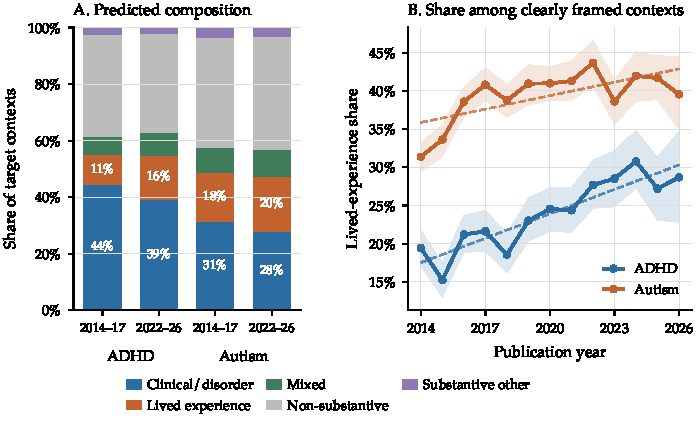
\includegraphics[width=\textwidth]{fig2_composition.pdf}
\end{center}
\caption{Frame composition of target contexts. Panel A compares the full predicted
composition in the early and late periods. Panel B gives the annual lived-experience share
among contexts assigned one clear frame, with 95\% document-bootstrap bands and OLS trend
summaries.}
\label{fig:composition}
\end{figure}

Across all 96{,}864 labelled contexts, clinical-only framing accounts for 42.1\% of ADHD
and 29.8\% of autism contexts and lived-only for 12.6\% and 18.8\%; the remainder are mixed
(7.0\%, 9.3\%), non-substantive (35.8\%, 38.8\%), and substantive-other (2.5\%, 3.3\%).

The composition moved (Figure~\ref{fig:composition}, Table~\ref{tab:composition}). Among
contexts assigned one clear frame, the lived-experience share of ADHD discourse rose by
1.07 percentage points per year ($p<.001$, adjusted $R^2 = .80$), a fitted increase from
17.5\% to 30.3\%. Autism moved the same way from a much higher base, 35.9\% to 42.9\%
($B = 0.59$, $p = .013$), but this series was flagged for residual autocorrelation and the
AR(1) sensitivity slope did not differ from zero ($p = .370$); we therefore treat the
autism compositional trend as unresolved and the ADHD one as robust.

\begin{table}[t!]
\caption{Annual trend models for the lived-experience share of clearly framed target
contexts, defined as lived-only divided by lived-only plus clinical-only.}
\label{tab:composition}
\small
\begin{tabular}{@{}lcccccc@{}}
\toprule
Target & $B$ (SE), pp/yr & $\beta$ & Adj. $R^2$ & Fitted 2014 & Fitted 2026 & AR(1) $B$ ($p$) \\
\midrule
ADHD & $1.07^{***}$ (0.15) & $+.90$ & $.80$ & 17.5\% & 30.3\% & --- \\
Autism & $0.59^{*\dagger}$ (0.20) & $+.67$ & $.39$ & 35.9\% & 42.9\% & $.23$ ($p = .370$) \\
\bottomrule
\end{tabular}
\par\vspace{3pt}
\parbox{\linewidth}{\footnotesize Note. $B$ is the annual OLS slope in percentage points;
$\beta$ is the standardised year coefficient. $^{\dagger}$ marks a residual-autocorrelation
flag, for which the AR(1) sensitivity slope is reported in the final column.
$^{*}p<.05$, $^{**}p<.01$, $^{***}p<.001$; $p$-values are descriptive and uncorrected.}
\end{table}


Because this trend is measured through a classifier, it is exposed to the possibility that
classifier error drifted over time. A period-stratified audit
(Appendix~\ref{app:stability}) finds the opposite of what that explanation requires:
lived-experience precision is \emph{highest} in the late period (.792, against .667 early),
and the human-adjudicated labels reproduce the rise independently of the classifier
(+1.11 percentage points per year, bootstrap 95\% CI [0.40, 1.88]). With only 11--23
lived-experience validation positives per period, modest error drift cannot be excluded and
the fitted 12.8-point rise may overstate the true change.

\subsection{No Vertical Creep}
\label{sec:vertical}

\begin{figure}[t!]
\begin{center}
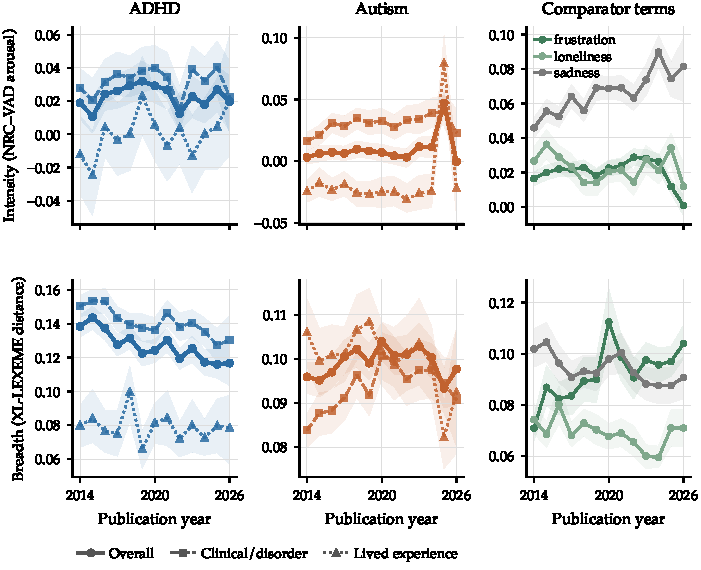
\includegraphics[width=\textwidth]{fig3_no_creep.pdf}
\end{center}
\caption{Annual intensity (top) and breadth (bottom) for the two targets by frame and for
the three comparator terms, with 95\% document-bootstrap bands. Neither predicted form of
concept creep appears: intensity does not decline, and breadth contracts rather than
broadens. The 2026 estimates rest on the thinnest annual samples, because each crawl
captures few pages published in its own year.}
\label{fig:nocreep}
\end{figure}

Intensity estimates rest on 17{,}649 ADHD and 39{,}463 autism contexts, of which 97.8\% and
99.3\% contributed at least one lexicon match, yielding 58{,}666 and 144{,}668 matched
collocate occurrences.

Vertical creep predicts declining arousal. It declined in no target stratum
(Table~\ref{tab:trends}, Figure~\ref{fig:nocreep}). For ADHD the slope did not differ from
zero overall ($B = 0.0001$, $p = .900$), in clinical contexts ($p = .738$), or in
lived-experience contexts ($p = .123$). For autism the overall slope was positive but not
distinguishable from zero ($p = .223$); the only slope that reached significance was a
nominal \emph{increase} in clinical contexts ($B = 0.0010$, $p = .048$), which is within
the range expected by chance across 34 tests and which we do not interpret. Given the
detectable-effect bound in Section~\ref{sec:stats}, the finding is that arousal did not
fall by more than about .013 (ADHD) or .022 (autism) index units over thirteen years.

\subsection{No Horizontal Creep---and Contraction}
\label{sec:horizontal}

Breadth estimates rest on 57{,}112 target contexts in the three substantive frames,
53{,}544 after within-cell duplicate removal, with 38{,}349 comparator rows.

Horizontal creep predicts increasing dispersion. Where breadth moved reliably, it moved the
other way. ADHD contracted overall, from .138 in 2014 to .117 in 2026
($B = -0.0020$, $p<.001$, adjusted $R^2 = .77$), and in clinical contexts
($B = -0.0018$, $p<.001$); these are the strongest semantic trends in the study. Autism
lived-experience breadth also declined ($B = -0.0010$, $p = .030$). Autism overall was flat
($p = .637$), and the nominally positive autism clinical slope ($p = .036$) was not retained
by the AR(1) model ($p = .755$).

\begin{table}[t!]
\caption{Annual trend models for the three semantic measures, by target and frame.
Sentiment and intensity are NRC--VAD valence and arousal over local collocates; breadth is
the mean pairwise cosine distance among XL-LEXEME target-use embeddings.}
\label{tab:trends}
\small
\begin{tabular}{@{}lllccc@{}}
\toprule
Measure & Target & Frame & $B$ (SE) & $\beta$ & Adj. $R^2$ \\
\midrule
Sentiment & ADHD & Overall & $.0023^{\dagger}$ (.0014) & $+.46$ & $.14$ \\
 & ADHD & Clinical & $.0013^{\dagger}$ (.0015) & $+.24$ & $-.03$ \\
 & ADHD & Lived experience & $.0002$ (.0017) & $+.03$ & $-.09$ \\
 & Autism & Overall & $.0012$ (.0006) & $+.50$ & $.18$ \\
 & Autism & Clinical & $.0022^{\dagger}$ (.0015) & $+.42$ & $.10$ \\
 & Autism & Lived experience & $-.0038$ (.0022) & $-.46$ & $.14$ \\
Intensity & ADHD & Overall & $.0001$ (.0005) & $+.04$ & $-.09$ \\
 & ADHD & Clinical & $.0002$ (.0006) & $+.10$ & $-.08$ \\
 & ADHD & Lived experience & $.0015$ (.0009) & $+.45$ & $.13$ \\
 & Autism & Overall & $.0011$ (.0008) & $+.36$ & $.05$ \\
 & Autism & Clinical & $.0010^{*}$ (.0004) & $+.56$ & $.25$ \\
 & Autism & Lived experience & $.0025$ (.0021) & $+.34$ & $.04$ \\
Breadth & ADHD & Overall & $-.0020^{***}$ (.0003) & $-.89$ & $.77$ \\
 & ADHD & Clinical & $-.0018^{***}$ (.0003) & $-.85$ & $.69$ \\
 & ADHD & Lived experience & $-.0004^{\dagger}$ (.0006) & $-.18$ & $-.06$ \\
 & Autism & Overall & $.0001^{\dagger}$ (.0002) & $+.14$ & $-.07$ \\
 & Autism & Clinical & $.0007^{*\dagger}$ (.0003) & $+.58$ & $.28$ \\
 & Autism & Lived experience & $-.0010^{*}$ (.0004) & $-.60$ & $.30$ \\
\bottomrule
\end{tabular}
\par\vspace{3pt}
\parbox{\linewidth}{\footnotesize Note. $B$ is the unstandardised annual OLS slope over 13
publication years; $\beta$ is the standardised year coefficient. $^{\dagger}$ marks a
residual-autocorrelation flag; AR(1) sensitivity estimates for flagged series are reported
in Appendix~\ref{app:ar1}. $^{*}p<.05$, $^{**}p<.01$, $^{***}p<.001$; $p$-values are
descriptive and uncorrected across 34 trend tests.}
\end{table}


A post-hoc diagnostic ranks contexts by their average distance to others in the same cell
(Appendix~\ref{app:posthoc}). The most distant ADHD contexts remain saturated with
diagnostic and educational vocabulary---\emph{disorder}, \emph{impulsivity},
\emph{inattention}, \emph{learning}, \emph{dyslexia}---rather than reaching into new
domains. That the comparator \emph{frustration} broadened over the
same window ($B = 0.0020$, $p<.01$) indicates the contraction is target-specific rather
than a corpus-wide artefact.

\subsection{Sentiment}

No target sentiment slope differed from zero in any stratum under the primary lexicon
(Table~\ref{tab:trends}). The autocorrelation-flagged series traced U-shapes with minima
between Q3 2018 and Q2 2019, and the AR(1) model gave a positive valence trend in autism
clinical contexts ($B = 0.0052$, $p = .040$). Quadratic coefficients are in
Appendix~\ref{app:quadratic}. We note the turning point but do not build on it: it rests on
diagnostics run because linear residuals were flagged, not on a pre-specified test.

\subsection{Operationalisation Sensitivity}
\label{sec:sensitivity}

\begin{figure}[t!]
\begin{center}
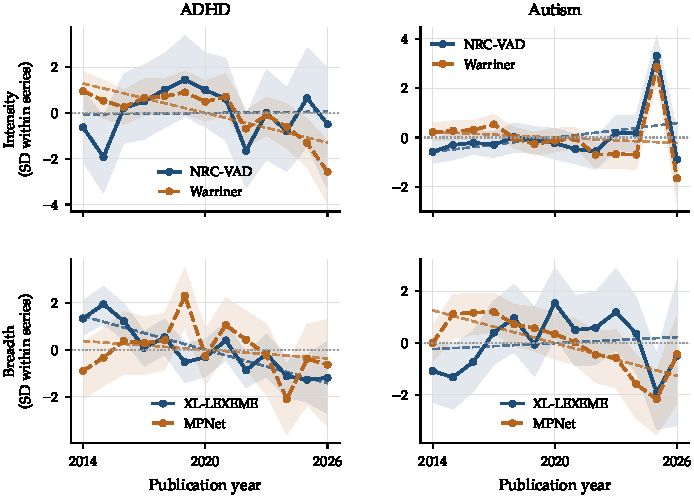
\includegraphics[width=\textwidth]{fig4_sensitivity.pdf}
\end{center}
\caption{The same series estimated under the primary and the original operationalisation.
Because the two affective lexicons use different native scales, each series is standardised
by its own across-year standard deviation; standardisation is a linear transform, so signs,
significance, and standardised slopes are exactly as reported in the trend tables. Dashed
lines are OLS fits.}
\label{fig:sensitivity}
\end{figure}

We now re-estimate every series with the resources SIBling originally specified.
Table~\ref{tab:concordance} asks, for each series, whether the two resources license the
same descriptive conclusion---the same significance verdict and, where significant, the
same sign. Fifteen of twenty-seven do not.

\begin{table}[t!]
\caption{Conclusion concordance across operationalisations. Each row asks whether the two
resources license the same descriptive conclusion for the same series: agreement requires
the same significance verdict at $p<.05$ and, where significant, the same sign.}
\label{tab:concordance}
\small
\begin{tabular}{@{}llccl@{}}
\toprule
Series & Frame & Primary $\beta$ & Alternative $\beta$ & Conclusion \\
\midrule
\multicolumn{5}{@{}l}{\itshape Sentiment: NRC--VAD versus Warriner} \\
ADHD & Overall & $+.46$ & $+.27$ & agree \\
ADHD & Clinical & $+.24$ & $-.14$ & agree \\
ADHD & Lived experience & $+.03$ & $-.19$ & agree \\
Autism & Overall & $+.50$ & $+.64^{*}$ & \textbf{differ} \\
Autism & Clinical & $+.42$ & $+.51$ & agree \\
Autism & Lived experience & $-.46$ & $-.30$ & agree \\
frustration & Baseline & $+.67^{*}$ & $+.64^{*}$ & agree \\
loneliness & Baseline & $+.71^{**}$ & $+.72^{**}$ & agree \\
sadness & Baseline & $-.79^{**}$ & $-.84^{***}$ & agree \\
\addlinespace
\multicolumn{5}{@{}l}{\itshape Intensity: NRC--VAD versus Warriner} \\
ADHD & Overall & $+.04$ & $-.80^{***}$ & \textbf{differ} \\
ADHD & Clinical & $+.10$ & $-.78^{**}$ & \textbf{differ} \\
ADHD & Lived experience & $+.45$ & $-.33$ & agree \\
Autism & Overall & $+.36$ & $-.14$ & agree \\
Autism & Clinical & $+.56^{*}$ & $-.38$ & \textbf{differ} \\
Autism & Lived experience & $+.34$ & $+.12$ & agree \\
frustration & Baseline & $-.23$ & $-.65^{*}$ & \textbf{differ} \\
loneliness & Baseline & $-.30$ & $-.73^{**}$ & \textbf{differ} \\
sadness & Baseline & $+.88^{***}$ & $+.23$ & \textbf{differ} \\
\addlinespace
\multicolumn{5}{@{}l}{\itshape Breadth: XL-LEXEME versus MPNet} \\
ADHD & Overall & $-.89^{***}$ & $-.23$ & \textbf{differ} \\
ADHD & Clinical & $-.85^{***}$ & $-.01$ & \textbf{differ} \\
ADHD & Lived experience & $-.18$ & $-.63^{*}$ & \textbf{differ} \\
Autism & Overall & $+.14$ & $-.79^{**}$ & \textbf{differ} \\
Autism & Clinical & $+.58^{*}$ & $-.09$ & \textbf{differ} \\
Autism & Lived experience & $-.60^{*}$ & $-.61^{*}$ & agree \\
frustration & Baseline & $+.72^{**}$ & $-.53$ & \textbf{differ} \\
loneliness & Baseline & $-.51$ & $-.81^{***}$ & \textbf{differ} \\
sadness & Baseline & $-.71^{**}$ & $+.27$ & \textbf{differ} \\
\bottomrule
\end{tabular}
\par\vspace{3pt}
\parbox{\linewidth}{\footnotesize Note. Cells report the standardised year coefficient,
which is comparable across resources on different native scales; raw slopes are not.
$^{*}p<.05$, $^{**}p<.01$, $^{***}p<.001$; $p$-values are descriptive and uncorrected. The
valence and arousal are scored on the same matched collocates within a lexicon, so the
sentiment and intensity blocks differ only in which rating is applied.}
\end{table}


The disagreement is concentrated by dimension rather than distributed across them.
Sentiment is close to invariant: eight of nine series agree, the exception being autism overall, which
sits either side of the threshold ($p = .081$ under NRC--VAD, $p = .018$ under Warriner).
Intensity fails in six of nine, and breadth in eight of nine. The two dimensions that carry
the concept-creep hypotheses are the two that do not survive substitution, while the
dimension we treated as exploratory is the one that does.

The individual disagreements are large. Under Warriner norms, ADHD intensity declines
reliably overall ($p = .001$) and in clinical contexts ($p = .002$) where NRC--VAD found
nothing---a result that, reported alone, would have been presented as textbook vertical
concept creep. The nominal autism clinical increase disappears ($p = .203$). Under MPNet,
the pronounced XL-LEXEME contraction in ADHD breadth attenuates to a null ($p = .445$) and
in ADHD clinical contexts vanishes entirely ($\beta = -0.01$, $p = .980$), while autism
overall breadth, flat under XL-LEXEME, becomes a reliable decline ($p = .001$).

The comparators rule out a target-specific explanation. If only the targets flipped, one
could argue these particular concepts are hard to measure. But \emph{sadness}, whose intensity rose
under NRC--VAD with the largest standardised coefficient in the comparator set
($\beta = +0.88$, $p<.001$), shows nothing under Warriner ($\beta = +0.23$, $p = .449$);
\emph{frustration} and \emph{loneliness}, null under NRC--VAD, both decline reliably under
Warriner; and for breadth all three comparators disagree across encoders, with
\emph{frustration} reversing from reliable broadening under XL-LEXEME to a non-significant
contraction under MPNet. The instruments reverse conclusions about ordinary emotion
vocabulary as readily as about diagnostic vocabulary.

One conclusion survives both operationalisations for both targets and can be stated with
corresponding confidence: \emph{neither target broadened horizontally}. Every reliable
breadth movement observed under either encoder is a contraction or a null. The
vertical-creep conclusion is measurement-conditional, and the sentiment conclusion holds for
every series except autism overall.

\subsection{Where the Disagreement Comes From}
\label{sec:mechanism}

Identifying the mechanism indicates which studies are at risk. For the lexicons it can be
isolated arithmetically; for the encoders it cannot, so we probe them behaviourally.

\subsubsection{Lexicons: ratings, not coverage}
Both lexicons were applied to the same collocate windows, so their matches share a context
index and can be crossed. Scoring the shared token set under each lexicon's ratings
separates the effect of \emph{which} tokens are scored from the effect of \emph{how} they
are scored. Table~\ref{tab:decomposition} reports the split.

\begin{table}[t!]
\caption{Why the affective lexicons disagree. The shift from the primary to the alternative
estimate is split into the part attributable to scoring a different set of tokens and the
part attributable to scoring shared tokens differently.}
\label{tab:decomposition}
\small
\begin{tabular}{@{}lccccc@{}}
\toprule
& \multicolumn{2}{c}{Standardised $\beta$} & \multicolumn{3}{c}{Decomposition of the shift} \\
\cmidrule(r){2-3}\cmidrule(l){4-6}
Series & NRC--VAD & Warriner & Total & Coverage & Ratings \\
\midrule
\multicolumn{6}{@{}l}{\itshape Valence (sentiment): NRC--VAD and Warriner ratings correlate $r = .89$ on shared vocabulary} \\
ADHD & $+.46$ & $+.27$ & $-.19$ & $+.01$ & $-.20$ \\
Autism & $+.50$ & $+.64$ & $+.14$ & $+.22$ & $-.08$ \\
frustration & $+.67$ & $+.64$ & $-.02$ & $+.05$ & $-.08$ \\
loneliness & $+.71$ & $+.72$ & $+.01$ & $+.06$ & $-.05$ \\
sadness & $-.79$ & $-.84$ & $-.05$ & $+.09$ & $-.14$ \\
\addlinespace
\multicolumn{6}{@{}l}{\itshape Arousal (intensity): NRC--VAD and Warriner ratings correlate $r = .62$ on shared vocabulary} \\
ADHD & $+.04$ & $-.80$ & $-.84$ & $+.26$ & $-1.11$ \\
Autism & $+.36$ & $-.14$ & $-.51$ & $+.08$ & $-.59$ \\
frustration & $-.23$ & $-.65$ & $-.41$ & $-.12$ & $-.30$ \\
loneliness & $-.30$ & $-.73$ & $-.43$ & $-.05$ & $-.38$ \\
sadness & $+.88$ & $+.23$ & $-.65$ & $-.05$ & $-.60$ \\
\bottomrule
\end{tabular}
\par\vspace{3pt}
\parbox{\linewidth}{\footnotesize Note. Both lexicons were applied to the same collocate
windows, so their matches can be crossed: the coverage column holds ratings fixed and varies
the token set, the ratings column holds the shared token set fixed and varies the rating.
Columns sum to the total up to a negligible interaction. Targets are the substantive
aggregate; comparators are unframed.}
\end{table}


Coverage does differ, and by more than a rounding error: NRC--VAD matches 866{,}246
collocate occurrences against Warriner's 801{,}639, with 87{,}164 occurrences (10.1\% of
the NRC total) invisible to Warriner, of which 18.5\% are multi-word entries the Warriner
norms cannot represent at all. Yet coverage explains little of the disagreement. Averaged
over series, the token set accounts for 11\% of the movement in the arousal estimate and
the ratings for 84\%; for ADHD the coverage term is $+0.26$ against a ratings term of
$-1.11$, so restricting NRC--VAD to Warriner's vocabulary leaves the conclusion essentially
unchanged while re-reading the same tokens with Warriner's numbers reverses it.

The reason is visible in the resources themselves. On the vocabulary they share, the two
lexicons agree closely about valence ($r = .89$ token-weighted, $.83$ type-level) and much
less about arousal ($r = .62$ on both). This makes the dimension-specific pattern in
Table~\ref{tab:concordance} interpretable rather than mysterious. Valence and arousal are
read off \emph{identical} matched collocates within a lexicon, so coverage is held exactly
constant between them and the only thing that changes is which rating is consulted.
Sentiment survives substitution and intensity does not because the field's two standard
affective resources substantially disagree about arousal while broadly agreeing about
valence. Any collocate-based intensity measure inherits that disagreement, whatever corpus
it is applied to.

\subsubsection{Encoders: what the representation is about}
Embeddings do not expose which tokens they scored, so no comparable decomposition is
available. Two observations stand in its place. First, the two encoders' annual breadth
estimates are close to unrelated: across the eleven series they correlate at mean
$r = +0.20$, and at $+0.11$ and $+0.17$ for the two overall target series, despite being
computed from nearly the same contexts. Whatever year-to-year variation one instrument
records, the other largely does not.

Second, we probed what each representation responds to. Taking 3{,}000 target contexts, we
built two minimally edited variants of each: one replacing the target term with the other
concept's term, and one replacing an unrelated content word. Table~\ref{tab:probe} reports
how far each encoder moves.

\begin{table}[t!]
\caption{What each breadth encoder responds to. Mean cosine distance between a context and
a minimally edited variant of it, over 3,000 target contexts.}
\label{tab:probe}
\small
\begin{tabular}{@{}lccc@{}}
\toprule
Encoder & Target swapped & Control word swapped & Ratio \\
\midrule
XL-LEXEME & $.1197$ & $.0009$ & $135$$\times$ \\
MPNet & $.1313$ & $.0106$ & $12$$\times$ \\
\bottomrule
\end{tabular}
\par\vspace{3pt}
\parbox{\linewidth}{\footnotesize Note. The target swap replaces the target term with the
other concept's term; the control swap replaces an unrelated content word in the same
context. Both conditions use the same contexts. A higher ratio means the representation is
more specific to the target and less contaminated by the rest of the sentence. Across the
11 annual series the two encoders' breadth estimates correlate at
mean $r = .20$.}
\end{table}


The result is not the one we predicted, and it is more informative. MPNet is not
insensitive to the target---it moves slightly further than XL-LEXEME when the target is
swapped ($.131$ against $.120$). The difference lies in what \emph{else} moves it. Swapping
an unrelated content word shifts XL-LEXEME by $.0009$, effectively nothing, but shifts
MPNet by $.0106$, an order of magnitude more. The ratio of target sensitivity to control
sensitivity is $135\times$ for XL-LEXEME against $12\times$ for MPNet.

This has a direct consequence for what breadth measures. Breadth is the dispersion of these
representations across a year's contexts. Under XL-LEXEME that dispersion is almost purely
dispersion in target usage, because little else appreciably moves the vector. Under MPNet it
also aggregates variation in whatever else the sentences contain---topic, register,
boilerplate---so the annual estimate is partly an index of how heterogeneous that year's
retained documents were. Two instruments presented as interchangeable operationalisations of
contextual breadth are therefore not measuring quite the same construct, and in a corpus
whose composition is itself changing they should not be expected to agree.

\section{Discussion}

\subsection{Grading the Evidence}

The paper's conclusions do not deserve equal confidence, and the comparison in
Section~\ref{sec:sensitivity} is what allows them to be graded. The useful result is that
the grading falls along dimensions rather than along findings: one measure is close to
invariant and two are not, for a reason that Section~\ref{sec:mechanism} identifies.

\emph{Robust to operationalisation.} Neither target broadened horizontally. This is one of
the two hypotheses the study set out to test, and no reliable broadening appears under
either encoder for either target. Sentiment is likewise close to invariant, agreeing in
eight of nine series.

\emph{Robust, and independently audited.} The compositional shift toward lived-experience
framing in ADHD discourse survives an AR(1) check, a period-stratified classifier audit,
independent reproduction in the human-adjudicated labels, and an unsupervised distributional
check on the frame distinction itself (Section~\ref{sec:frames}).

\emph{Measurement-conditional.} The vertical-creep conclusion depends on the affective
lexicon. Under our primary measure intensity is flat; under the framework's original measure
ADHD intensity declines reliably. We prefer NRC--VAD on coverage and reliability grounds
\citep{mohammadNRCVADLexicon2025}, but that is an \emph{a priori} argument and does not
dissolve the empirical problem. The honest statement is that vertical creep for ADHD cannot
presently be adjudicated with these instruments---and, given that the two standard resources
correlate at only $r = .62$ on arousal, that limitation is not specific to this study.

\emph{Directionally suggestive, not established.} The ADHD breadth contraction is the
largest effect observed, but breadth is also the least invariant dimension, and the probe in
Section~\ref{sec:mechanism} shows the two encoders are not measuring quite the same thing.

\subsection{Composition Is Not Meaning}

Frame stratification earned its cost, and the corpus allows the reason to be quantified
rather than asserted. \citet{pislRevisitingSemanticSeverity2025} and
\citet{xiaoHaveConceptsAnxiety2023} warn that a measured affective trend can be produced by
a changing mixture of contexts: if clinical contexts are more intense than non-clinical
ones, then a corpus drifting toward clinical language will show rising intensity, and one
drifting away from it will show falling intensity, whatever happens to the meaning of the
term. Both conditions hold here. Clinical contexts are markedly higher in arousal than
lived-experience contexts---averaging the first and last year, .025 against .004 for ADHD
and .020 against $-.023$ for autism---and the mixture moved: the clinical share of
substantive ADHD contexts fell from 72.3\% to 63.9\% while the lived-experience share rose
from 17.4\% to 25.7\%.

Decomposing the change in the aggregate arousal index into a within-frame and a
compositional component makes the consequence explicit. For autism the aggregate fell by
.0033 across the window, of which $-.0036$ is compositional and $+.0003$ within-frame:
essentially the whole apparent decline is the mixture moving, not the frames. For ADHD the
two components have opposite signs---composition $-.0018$, within-frame $+.0035$---and
nearly cancel, leaving the flat aggregate the paper reports. Note the sign: the mixture
here moved \emph{away} from clinical framing, so what the frame series record is the
converse of pathologisation rather than pathologisation itself.

This is the Písl and Xiao mechanism operating in the direction that favours the hypothesis
under test. An unstratified analysis of this corpus would have found aggregate arousal
drifting downward for autism and would have been entitled, on the usual reasoning, to call
it vertical concept creep. The stratified analysis shows the frames themselves did not
soften. Our null is therefore conservative: it survives a compositional trend that was
pushing the aggregate toward the creep prediction. The same decomposition applies to the
valence result, where roughly 40 to 45\% of the apparent improvement is compositional rather
than a change within either frame.

The composition problem also differs in kind from the one Písl and Xiao address. For
\emph{anxiety} or \emph{depression}, stratification must first separate the clinical
construct both from ordinary states---everyday anxiety before an exam, feeling depressed
after bad news---and from unrelated senses, such as an economic depression or a
meteorological one \citep{xiaoHaveConceptsAnxiety2023}. ADHD and autism are diagnostic by
definition, so no sense disambiguation is needed, and yet composition still shifts, because
what changes is the \emph{framing} of the diagnosis, from disorder construct to identity and
lived experience. Composition confounding is therefore not a special problem of polysemous
targets; it arises wherever the discourse around a stable referent is itself in motion.

\subsection{Semantic Consolidation Rather Than Creep}

The substantive pattern is a double null with a directional surprise: ADHD and autism did
not drift into milder contexts, did not disperse across a wider range of them, and remained
thematically anchored to diagnosis, childhood, and family, while the clearest movement ran
toward contraction.

This is intelligible alongside \citeauthor{iacobComputationalAnalysisEmergence2026}'s
\citeyear{iacobComputationalAnalysisEmergence2026} finding that long-established, codified
terms such as \emph{OCD} and \emph{bipolar} moved little on Reddit while newer vernacular
terms shifted substantially. ADHD and autism are institutionally anchored: their reference
is stabilised by diagnostic manuals, clinical gatekeeping, service categories, and
educational law in ways that ordinary-language harm concepts such as \emph{bullying} or
\emph{harassment} \citep{vylomovaSemanticChangesHarmrelated2021} are not. This suggests a
distinction the creep literature has tended to elide. A category can expand
\emph{extensionally}, admitting many more people---as ADHD's diagnostic criteria did across
successive DSM revisions \citep{fabianoDiagnosticInflationDSM2020,americanpsychiatricassociationDiagnosticStatisticalManual2013}---while
the typical linguistic contexts of its name, which is all that collocate- and
embedding-based measures index, hold their shape. Rising diagnosed prevalence
\citep{zeidanGlobalPrevalenceAutism2022,mckechnieAttentiondeficitHyperactivityDisorder2023}
need not leave the semantic trace a direct reading of concept creep would predict.

What did change is who is talking and in what register. The shift from clinical toward
lived-experience framing, much sharper for ADHD, is consistent with the recent growth of
adult self-recognition and identity-oriented content
\citep{ginappExperiencesAdultsADHD2023,alperTikTokAlgorithmicallyMediated2025,martinChangingPrevalenceADHD2025},
and with autism having partly completed that reframing earlier, which would leave its trend
flatter---as we find. For the trivialisation concern that motivates much of this literature
\citep{isern-masUnmaskingTherapyspeak2025,spencerIsntEveryoneLittle2021}, the semantic
preconditions are not in evidence in this corpus: the words largely held their shape; the
conversation around them did not.

\subsection{Implications for LSC Practice}
\label{sec:practice}

Three recommendations follow, in decreasing order of confidence.

\emph{Treat multi-resource comparison as primary, not supplementary.} On our evidence a
single-resource LSC study reports the properties of a resource as though they were
properties of a concept. The remedy is cheap: estimating every trajectory twice cost one
additional pass over an existing pipeline, and it converted an unqualified claim about
vertical creep into a correctly hedged one. Where two resources disagree, the disagreement
is the finding.

Concretely, this suggests a minimal reporting protocol that any study in this tradition
could adopt without new data. Estimate each dimension under at least two defensible
resources and report both. Compare them on sign, significance, and standardised effect
rather than raw magnitude, since resources on different native scales are not otherwise
commensurable. Where resources disagree, check whether they disagree about which
tokens to score or about how to score them: Section~\ref{sec:mechanism} shows the two have
very different implications, and the check costs one join. Finally, state a conclusion at
the strength the weakest concordant resource supports, and mark measurement-conditional
findings as such rather than selecting the resource with the cleaner result.

\emph{Stratify before estimating.} Composition should be modelled explicitly whenever the
discourse around a term may be changing, which for socially contested vocabulary is
routine. Our classifier is one way to do this; a topic model, a genre classifier, or even
recorded metadata strata would serve, and the choice matters less than making one. The
general point is that the analyst must decide what population the trend is a trend
\emph{in}, and that leaving this implicit does not make the decision go away---it makes it
the corpus's decision rather than the analyst's.

\emph{Validate the dimensions against human judgement.} Neither intensity, breadth, nor
connotation as operationalised in this tradition has been benchmarked against human ratings
of the same contexts. Until that exists, resource choice rests on plausibility arguments of
the kind we ourselves make in Section~\ref{sec:alternatives}, and non-invariance of the
kind documented here cannot be adjudicated. This is the most consequential gap our results
expose.

\subsection{Limitations}

The corpus is the most consequential limitation. Common Crawl's coverage is shaped by
harmonic centrality, absent social platforms, and growing \texttt{robots.txt} blocking over
exactly our window \citep{baackCriticalAnalysisLargest2024}. Findings generalise to quality-filtered English open-web
discourse as archived by Common Crawl, not to public discourse at large, and emphatically
not to the platforms where much contemporary ADHD and autism discourse now occurs. The
final year is also the thinnest, since each crawl captures few pages published in its own
year, so 2026 estimates are the least stable in every series.

The frame design inherits classifier error, and the weakest head is the one carrying the
headline compositional result; the temporal-stability audit constrains but does not
eliminate this. All human labels come from one coder, so no inter-annotator agreement can
be reported. The affective measures score lemmatised collocates with
context-free lexicon values and are blind to negation, irony, and syntactic scope. The
comparators are baselines for negative-affect language, not matched controls in the sense
\citet{dubossarsky-etal-2017-outta} recommend. And the design is observational: it
characterises how discourse changed, not why.

Finally, the scope of the measurement claim should not be overstated. We demonstrate
non-invariance in one well-instrumented case, across two resource substitutions, two
targets, three comparators, and three frame strata. That the comparator conclusions flip
too makes an idiosyncratic explanation unlikely, but we do not estimate how general the
problem is across dimensions, resources, or corpora. Establishing that is the natural next
study.

\section{Conclusion}

We asked whether measured lexical semantic change survives the choices that produce it.
Applied to a 13-year web corpus, it depends on the dimension: fifteen of twenty-seven series
change their descriptive conclusion when the framework's own alternative lexicon and encoder
are substituted, and the reversals reach ordinary emotion vocabulary as readily as diagnostic
vocabulary. Sentiment is close to invariant; intensity and breadth are not. Neither failure
is mysterious. The two standard affective lexicons agree about valence and disagree about
arousal on the very same tokens, so a collocate-based intensity measure inherits a
disagreement that has nothing to do with the corpus; and the two standard encoders differ by
an order of magnitude in how much non-target material moves them, so their dispersion
estimates are not measuring quite the same construct.

The substantive findings are graded accordingly. Neither predicted form of concept creep is
supported for ADHD or autism, with the null bounded and, on the shift-share evidence,
conservative---the corpus composition was moving in the direction that manufactures apparent
vertical creep, and the frames themselves still did not soften. The horizontal result is
robust to operationalisation while the vertical one is not, and the clearest change over the
period is compositional, a shift from clinical toward lived-experience framing that survives
independent audit.

The methodological implication is modest to state and inconvenient to adopt. If a field
intends to infer cultural change from lexical measurement, it must first show that the
measurement is stable under substitutions its own practitioners regard as innocuous, and
diagnose the substitutions that are not. Doing so costs one extra pass over an existing
pipeline. Not doing so risks reporting the properties of a lexicon as the properties of a
culture.

\begin{acknowledgments}
I thank Dr Tom Paskhalis for his supervision of the research on which this paper is based.
\end{acknowledgments}

\appendix

\appendixsection{Classifier Temporal-Stability Audit}
\applabel{app:stability}

Table~\ref{tab:stability} reports held-out validation performance for the frozen classifier
stratified by period, from the post-hoc audit of the compositional trend in
Section~\ref{sec:composition}. Periods follow the corpus banding, which balances the
200-passage validation set at 67/67/66. Clinical recall is nominally lower in the late
period, but lived-experience error rates are homogeneous across periods and
lived-experience precision is highest late---the opposite of the pattern that drifting
classifier error would need in order to manufacture the observed rise.

\begin{table}[t!]
\centering
\caption{Period-stratified held-out validation performance for the hierarchical frame classifier. Brackets give 95\% Clopper--Pearson intervals; F1 intervals are stratified bootstrap percentiles.}
\label{tab:stability}
\small
\begin{tabular}{@{}lccccc@{}}
\toprule
Period & Support & Precision & Recall & FPR & F1 \\
\midrule
\multicolumn{6}{@{}l}{\itshape Substantive target discourse} \\
2014--2017 & 45/67 & .884 [.75, .96] & .844 [.71, .94] & .227 [.08, .45] & .864 [.78, .93] \\
2018--2022 & 46/67 & .816 [.68, .91] & .870 [.74, .95] & .429 [.22, .66] & .842 [.76, .91] \\
2023--2026 & 50/66 & .976 [.87, 1.00] & .800 [.66, .90] & .062 [.00, .30] & .879 [.80, .94] \\
\addlinespace
\multicolumn{6}{@{}l}{\itshape Clinical framing} \\
2014--2017 & 36/45 & .897 [.76, .97] & .972 [.85, 1.00] & .444 [.14, .79] & .933 [.87, .99] \\
2018--2022 & 37/46 & .971 [.85, 1.00] & .892 [.75, .97] & .111 [.00, .48] & .930 [.86, .99] \\
2023--2026 & 32/50 & .833 [.65, .94] & .781 [.60, .91] & .278 [.10, .53] & .806 [.68, .90] \\
\addlinespace
\multicolumn{6}{@{}l}{\itshape Lived-experience framing} \\
2014--2017 & 11/45 & .667 [.35, .90] & .727 [.39, .94] & .118 [.03, .27] & .696 [.43, .88] \\
2018--2022 & 12/46 & .611 [.36, .83] & .917 [.62, 1.00] & .206 [.09, .38] & .733 [.53, .89] \\
2023--2026 & 23/50 & .792 [.58, .93] & .826 [.61, .95] & .185 [.06, .38] & .809 [.67, .92] \\
\bottomrule
\end{tabular}
\parbox{\linewidth}{\footnotesize Note. Support gives positive cases over the per-period evaluation denominator. Substantive target discourse is evaluated on all held-out passages in the period; clinical and lived-experience framing are evaluated among human-substantive passages, following the aggregate validation convention. FPR = false-positive rate.}
\end{table}


\appendixsection{Comparator Trend Models}
\applabel{app:comparators}

Table~\ref{tab:comparators} reports the unframed comparator trend models used to
contextualise the target trajectories, across all four measures.

\input{../reports/tables/cl/appx_comparators.tex}

\appendixsection{AR(1) Sensitivity Models}
\applabel{app:ar1}

Table~\ref{tab:ar1} reports first-order autoregressive sensitivity estimates for every
series flagged for residual autocorrelation in the main tables.

\begin{table}[t!]
\centering
\caption{AR(1) sensitivity models for autocorrelation-flagged annual series.}
\label{tab:ar1}
\scriptsize
\begin{tabular}{@{}llllccc@{}}
\toprule
Source & Measure & Series & Frame & OLS $B$ & AR(1) $B$ & AR(1) $p$ \\
\midrule
Table~\ref{tab:trends} & Sentiment & ADHD & Overall & $0.0023$ & $0.0037$ & $.147$ \\
Table~\ref{tab:trends} & Sentiment & ADHD & Clinical & $0.0013$ & $0.0036$ & $.218$ \\
Table~\ref{tab:trends} & Sentiment & Autism & Clinical & $0.0022$ & $0.0052$ & $.040$ \\
Table~\ref{tab:trends} & Breadth & ADHD & Lived experience & $-0.0004$ & $-0.0004$ & $.247$ \\
Table~\ref{tab:trends} & Breadth & Autism & Overall & $0.0001$ & $-0.0001$ & $.753$ \\
Table~\ref{tab:trends} & Breadth & Autism & Clinical & $0.0007$ & $0.0002$ & $.755$ \\
Table~\ref{tab:composition} & Frame classification & Autism & Lived vs clinical & $0.59$ & $0.23$ & $.370$ \\
Table~\ref{tab:comparators} & Salience & frustration & Baseline & $-0.0175$ & $0.0160$ & $.538$ \\
Table~\ref{tab:comparators} & Sentiment & frustration & Baseline & $0.0037$ & $0.0116$ & $.003$ \\
Table~\ref{tab:comparators} & Sentiment & loneliness & Baseline & $0.0044$ & $0.0070$ & $.009$ \\
Table~\ref{tab:comparators} & Intensity & frustration & Baseline & $-0.0004$ & $-0.0022$ & $.078$ \\
Table~\ref{tab:comparators} & Breadth & sadness & Baseline & $-0.0010$ & $-0.0008$ & $.131$ \\
\bottomrule
\end{tabular}
\parbox{\linewidth}{\footnotesize Note. Rows are the series marked with $^{\dagger}$ in the compact regression tables. OLS $B$ repeats the primary annual slope; AR(1) $B$ reports the first-order autoregressive sensitivity slope for the same series. The frame-classification row is reported in percentage points per year; all other rows use the original index units per year. P values are descriptive and uncorrected.}
\end{table}


\appendixsection{Quadratic Trend Diagnostics}
\applabel{app:quadratic}

Table~\ref{tab:quadratic} reports quadratic models for the annual series whose linear
residuals were flagged. These are diagnostics run because of a residual check, not
pre-specified tests, and are reported for completeness rather than as competing trend
estimates.

\input{../reports/tables/cl/appx_quadratic.tex}

\appendixsection{Post-hoc Contributor Diagnostics}
\applabel{app:posthoc}

Tables~\ref{tab:posthoc-sentiment}--\ref{tab:posthoc-breadth} summarise which collocates
carry the valence and arousal estimates, and which content words characterise the
highest-distance breadth contexts, grouped into early, middle, and late periods. These are
descriptive aids to interpretation, computed after the annual analyses.

\input{../reports/tables/cl/appx_posthoc_sentiment.tex}
\begin{table}[t!]
\centering
\caption{Post-hoc arousal collocate contributors by target, frame, and period.}
\label{tab:posthoc-arousal}
\scriptsize
\setlength{\tabcolsep}{3.5pt}
\renewcommand{\arraystretch}{1.2}
\begin{tabular}{@{}llp{0.235\linewidth}p{0.235\linewidth}p{0.235\linewidth}@{}}
\toprule
Target & Frame & 2014-2017 & 2018-2021 & 2022-2026 \\
\midrule
ADHD & Overall & \begin{minipage}[t]{\linewidth}\raggedright Raising: disorder, anxiety, hyperactivity\\ Lowering: add, treatment, patient\end{minipage} & \begin{minipage}[t]{\linewidth}\raggedright Raising: anxiety, disorder, hyperactivity\\ Lowering: add, sleep, student\end{minipage} & \begin{minipage}[t]{\linewidth}\raggedright Raising: anxiety, disorder, challenge\\ Lowering: individual, common, treatment\end{minipage} \\
ADHD & Clinical & \begin{minipage}[t]{\linewidth}\raggedright Raising: disorder, anxiety, hyperactivity\\ Lowering: treatment, add, patient\end{minipage} & \begin{minipage}[t]{\linewidth}\raggedright Raising: disorder, anxiety, hyperactivity\\ Lowering: add, sleep, narcolepsy\end{minipage} & \begin{minipage}[t]{\linewidth}\raggedright Raising: anxiety, disorder, hyperactivity\\ Lowering: treatment, common, individual\end{minipage} \\
ADHD & Lived experience & \begin{minipage}[t]{\linewidth}\raggedright Raising: anxiety, suffer, struggle\\ Lowering: parent, student, add\end{minipage} & \begin{minipage}[t]{\linewidth}\raggedright Raising: anxiety, challenge, disorder\\ Lowering: student, add, dyslexia\end{minipage} & \begin{minipage}[t]{\linewidth}\raggedright Raising: challenge, anxiety, struggle\\ Lowering: autistic, dyslexia, individual\end{minipage} \\
Autism & Overall & \begin{minipage}[t]{\linewidth}\raggedright Raising: disorder, developmental, spectrum\\ Lowering: link, family, individual\end{minipage} & \begin{minipage}[t]{\linewidth}\raggedright Raising: disorder, developmental, spectrum\\ Lowering: people, individual, family\end{minipage} & \begin{minipage}[t]{\linewidth}\raggedright Raising: disorder, developmental, dangerous\\ Lowering: individual, people, family\end{minipage} \\
Autism & Clinical & \begin{minipage}[t]{\linewidth}\raggedright Raising: disorder, developmental, schizophrenia\\ Lowering: link, center, individual\end{minipage} & \begin{minipage}[t]{\linewidth}\raggedright Raising: disorder, developmental, spectrum\\ Lowering: link, individual, center\end{minipage} & \begin{minipage}[t]{\linewidth}\raggedright Raising: disorder, developmental, schizophrenia\\ Lowering: individual, therapy, link\end{minipage} \\
Autism & Lived experience & \begin{minipage}[t]{\linewidth}\raggedright Raising: disorder, boy, spectrum\\ Lowering: son, family, people\end{minipage} & \begin{minipage}[t]{\linewidth}\raggedright Raising: disorder, challenge, spectrum\\ Lowering: people, son, individual\end{minipage} & \begin{minipage}[t]{\linewidth}\raggedright Raising: dangerous, obsession, disorder\\ Lowering: individual, people, family\end{minipage} \\
\bottomrule
\end{tabular}
\parbox{\linewidth}{\footnotesize Note. Cells show the three largest preprocessed collocate contributors from each direction.}
\end{table}
\input{../reports/tables/cl/appx_posthoc_breadth.tex}

\appendixsection{Post-hoc Diagnostic on the Frame Distinction}
\applabel{app:thematic}

This appendix supports the post-hoc diagnostic reported in Section~\ref{sec:frames}.
Skip-gram models with 200-dimensional vectors, a context window of 10, a minimum count of
5, and 10 epochs are trained per target-frame corpus and warm-started per publication year,
following \citet{vylomovaSemanticChangesHarmrelated2021}. A neighbour is retained only if
the canonical target token occurs at least 20 times in the relevant cell, the neighbour
occurs at least five times, it enters an annual top-five list in at least two years, and it
has finite estimates in at least ten of the thirteen years. Of 390 annual neighbour rows,
28 neighbours and 364 annual estimates survive.

\begin{figure}[t!]
\begin{center}
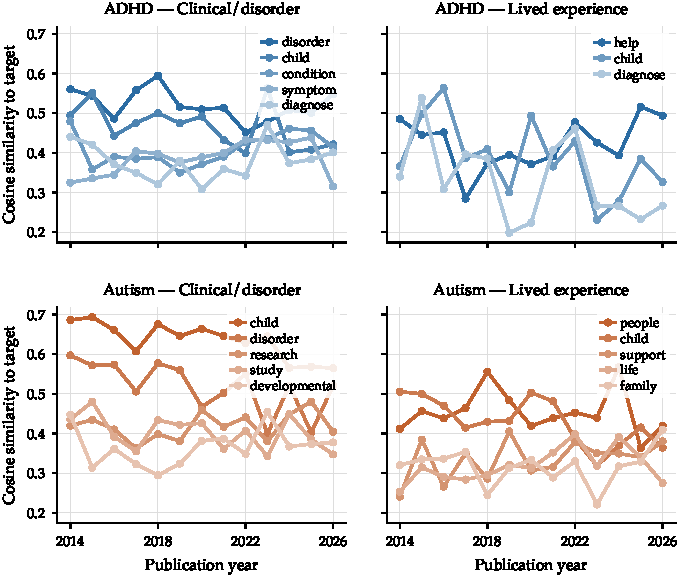
\includegraphics[width=\textwidth]{figF1_neighbours.pdf}
\end{center}
\caption{Annual cosine similarity between each target concept token and its stable
distributional neighbours, within the clinical and lived-experience frames. Neighbours are
ordered in each legend by mean similarity. The overall stratum is omitted: pooling the
frames answers a different question from the one this diagnostic asks.}
\label{fig:thematic}
\end{figure}

Figure~\ref{fig:thematic} shows the contrast Section~\ref{sec:frames} draws on. Within
autism the two panels barely overlap: the clinical frame is anchored by \emph{developmental},
\emph{disorder}, \emph{research}, and \emph{study}, the lived-experience frame by
\emph{family}, \emph{life}, \emph{people}, and \emph{support}. ADHD separates less sharply,
with \emph{disorder}, \emph{symptom}, and \emph{condition} against \emph{help}, which is
consistent with the classifier's weaker lived-experience head. The surviving neighbours also
stay diagnostic and child- or family-centred across the whole window, but we do not draw
that second conclusion here: annual models fitted to yearly slices are known to be unstable
\citep{antoniak-mimno-2018-evaluating}, so these trajectories are used only to establish
that the two frames occupy different distributional neighbourhoods, not to estimate how
those neighbourhoods changed over time.

\bibliographystyle{compling}
\bibliography{bibs/cl-short-paper}

\end{document}
